\documentclass[11pt,a4paper]{article}
\usepackage[utf8]{inputenc}
\usepackage[margin=1in]{geometry}
\usepackage{xcolor}
\usepackage{booktabs}
\usepackage{longtable}
\usepackage{graphicx}
\usepackage{tikz}
\usetikzlibrary{shapes,arrows,positioning}

% Define colors
\definecolor{mongogreen}{RGB}{0,104,56}
\definecolor{postgresblue}{RGB}{50,103,145}
\definecolor{redisred}{RGB}{220,47,2}

\title{\textbf{Serenify Database Architecture}}
\author{SALVIORIS Development Team}
\date{\today}

\begin{document}

\maketitle

\section{Overview}

Serenify employs a hybrid database architecture utilizing three distinct database systems, each optimized for specific use cases:

\begin{itemize}
    \item \textcolor{mongogreen}{\textbf{MongoDB}} --- Document-oriented storage for unstructured content
    \item \textcolor{postgresblue}{\textbf{PostgreSQL}} --- Relational storage for structured user data
    \item \textcolor{redisred}{\textbf{Redis}} --- In-memory caching and real-time messaging
\end{itemize}

\section{Database Distribution}

\subsection{\textcolor{mongogreen}{MongoDB Collections}}

MongoDB is used for storing user-generated content that benefits from flexible schemas and document-based storage.

\begin{longtable}{|p{4cm}|p{10cm}|}
\hline
\rowcolor{mongogreen!20}
\textbf{Collection} & \textbf{Purpose} \\
\hline
\endfirsthead

\hline
\rowcolor{mongogreen!20}
\textbf{Collection} & \textbf{Purpose} \\
\hline
\endhead

\texttt{vents} & Anonymous emotional venting posts. Stores user messages with optional user association (supports both logged-in and anonymous users). \\
\hline

\texttt{journals} & Private journaling entries. Each entry contains a title, content, and is associated with a specific user via \texttt{user\_id\_string}. \\
\hline

\texttt{therapists} & Therapist profiles including credentials, license information, education, specialization, and approval status. Stores certificate and degree image paths. \\
\hline

\texttt{feedback} & User feedback submissions. Stores feedback content and optional IP address for analytics. \\
\hline

\texttt{chat\_messages} & Real-time chat message persistence. Stores group chat messages with sender information, timestamps, and delivery status. Indexed by \texttt{(group\_id, timestamp)} for efficient pagination. \\
\hline

\end{longtable}

\subsection{\textcolor{postgresblue}{PostgreSQL Tables}}

PostgreSQL handles structured relational data requiring ACID compliance, complex queries, and referential integrity.

\begin{longtable}{|p{4cm}|p{10cm}|}
\hline
\rowcolor{postgresblue!20}
\textbf{Table} & \textbf{Purpose} \\
\hline
\endfirsthead

\hline
\rowcolor{postgresblue!20}
\textbf{Table} & \textbf{Purpose} \\
\hline
\endhead

\texttt{users} & Core user accounts. Stores username, password hash, creation timestamp, and active status. \\
\hline

\texttt{user\_recovery} & Encrypted recovery data. Stores encrypted email and phone numbers for account recovery purposes. \\
\hline

\texttt{user\_devices} & Device tracking for security. Records device tokens, IP addresses, user agents, and last usage timestamps. \\
\hline

\texttt{violations} & Content moderation violations. Tracks threats, self-harm content, and associated actions taken (warnings, blocks). \\
\hline

\texttt{blocked\_ips} & IP address blacklist. Manages temporary and permanent IP blocks with expiration timestamps. \\
\hline

\texttt{password\_reset\_tokens} & Password recovery tokens. Stores time-limited tokens for secure password reset flows. \\
\hline

\texttt{feedbacks} & Duplicate feedback storage in PostgreSQL for relational querying and analytics. \\
\hline

\texttt{contact\_us} & Contact form submissions. Stores user inquiries and support requests. \\
\hline

\texttt{user\_waitlist} & User registration waitlist. Manages early access requests. \\
\hline

\texttt{therapist\_waitlist} & Therapist registration waitlist. Manages therapist onboarding queue. \\
\hline

\texttt{admins} & Administrative user accounts with elevated privileges. \\
\hline

\texttt{groups} & Chat group metadata. Stores group names, descriptions, creation timestamps, and creator information. \\
\hline

\texttt{group\_members} & Group membership relationships. Many-to-many relationship between users and groups with join timestamps. \\
\hline

\texttt{group\_messages} & Relational storage of group messages (complementary to MongoDB). Provides structured querying capabilities. \\
\hline

\texttt{activity\_events} & User activity logging. Tracks user actions for analytics and audit trails. \\
\hline

\end{longtable}

\subsection{\textcolor{redisred}{Redis Usage}}

Redis provides high-performance in-memory storage for caching and real-time features.

\begin{longtable}{|p{4cm}|p{10cm}|}
\hline
\rowcolor{redisred!20}
\textbf{Use Case} & \textbf{Purpose} \\
\hline
\endfirsthead

\hline
\rowcolor{redisred!20}
\textbf{Use Case} & \textbf{Purpose} \\
\hline
\endhead

\texttt{Session Caching} & Stores user session tokens and authentication state for fast validation. \\
\hline

\texttt{Chat Cache} & Caches recent chat messages for instant retrieval, reducing MongoDB query load. \\
\hline

\texttt{Real-time Pub/Sub} & Facilitates WebSocket message broadcasting for live chat functionality. \\
\hline

\texttt{Rate Limiting} & Implements API rate limiting using Redis counters with TTL. \\
\hline

\end{longtable}

\section{Architecture Diagram}

\begin{center}
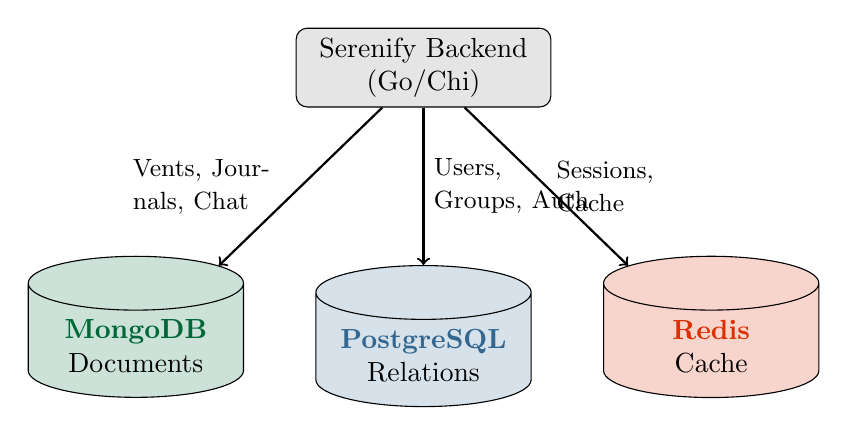
\begin{tikzpicture}[
    node distance=2cm,
    box/.style={rectangle, draw, fill=blue!10, text width=3cm, text centered, rounded corners, minimum height=1cm},
    db/.style={cylinder, draw, shape border rotate=90, aspect=0.25, text width=2.5cm, text centered, minimum height=1.5cm}
]

% Application Layer
\node[box, fill=gray!20] (app) {Serenify Backend\\(Go/Chi)};

% Databases
\node[db, fill=mongogreen!20, below left=2cm and 1cm of app] (mongo) {\textcolor{mongogreen}{\textbf{MongoDB}}\\Documents};
\node[db, fill=postgresblue!20, below=2cm of app] (postgres) {\textcolor{postgresblue}{\textbf{PostgreSQL}}\\Relations};
\node[db, fill=redisred!20, below right=2cm and 1cm of app] (redis) {\textcolor{redisred}{\textbf{Redis}}\\Cache};

% Arrows
\draw[->, thick] (app) -- node[left, text width=2cm] {\small Vents, Journals, Chat} (mongo);
\draw[->, thick] (app) -- node[right, text width=2cm] {\small Users, Groups, Auth} (postgres);
\draw[->, thick] (app) -- node[right, text width=2cm] {\small Sessions, Cache} (redis);

\end{tikzpicture}
\end{center}

\section{Design Rationale}

\subsection{MongoDB for Content}
\begin{itemize}
    \item \textbf{Flexible Schema}: User-generated content (vents, journals) varies in structure
    \item \textbf{Horizontal Scaling}: Document-based storage scales easily for high-volume writes
    \item \textbf{JSON-native}: Natural fit for REST API responses
\end{itemize}

\subsection{PostgreSQL for Structure}
\begin{itemize}
    \item \textbf{ACID Compliance}: Critical for user authentication and financial transactions
    \item \textbf{Complex Queries}: Supports joins for group membership and analytics
    \item \textbf{Referential Integrity}: Enforces foreign key constraints for data consistency
\end{itemize}

\subsection{Redis for Performance}
\begin{itemize}
    \item \textbf{Sub-millisecond Latency}: Essential for session validation and rate limiting
    \item \textbf{Pub/Sub}: Enables real-time WebSocket message distribution
    \item \textbf{TTL Support}: Automatic expiration for temporary data (sessions, tokens)
\end{itemize}

\section{Data Flow Examples}

\subsection{User Creates a Vent}
\begin{enumerate}
    \item User authenticates (session validated via \textcolor{redisred}{Redis})
    \item User ID retrieved from \textcolor{postgresblue}{PostgreSQL} \texttt{users} table
    \item Vent document inserted into \textcolor{mongogreen}{MongoDB} \texttt{vents} collection
    \item Moderation check performed (violations logged to \textcolor{postgresblue}{PostgreSQL})
\end{enumerate}

\subsection{User Joins Chat Group}
\begin{enumerate}
    \item User authentication via \textcolor{redisred}{Redis} session
    \item Group membership inserted into \textcolor{postgresblue}{PostgreSQL} \texttt{group\_members}
    \item Recent messages loaded from \textcolor{redisred}{Redis} cache
    \item Older messages fetched from \textcolor{mongogreen}{MongoDB} \texttt{chat\_messages}
    \item Real-time updates via \textcolor{redisred}{Redis} Pub/Sub
\end{enumerate}

\section{Summary}

The Serenify platform leverages a polyglot persistence strategy:
\begin{itemize}
    \item \textcolor{mongogreen}{\textbf{5 MongoDB collections}} for flexible content storage
    \item \textcolor{postgresblue}{\textbf{15 PostgreSQL tables}} for structured relational data
    \item \textcolor{redisred}{\textbf{Redis}} for caching and real-time features
\end{itemize}

This architecture ensures optimal performance, scalability, and data integrity across all platform features.

\end{document}
